\documentclass[11pt]{article}

\usepackage[a4paper,margin=1in,footskip=.3in]{geometry}

\usepackage{fancyhdr}
\pagestyle{fancy}

\setlength\headheight{15pt}

\rhead{October 2014}
\chead{\textsc{Research Notes}}
\lhead{\textsc{Louis Tiao}}
\rfoot{\textsc{\thepage}}
\cfoot{\textit{Last modified: \today}}

\usepackage{float}
\usepackage{wrapfig}
\usepackage{graphicx}
\graphicspath{{../../figures/}}
\usepackage{cleveref}
\usepackage{hyperref}
\hypersetup{
    colorlinks,
    citecolor=black,
    filecolor=black,
    linkcolor=black,
    urlcolor=black
}
\usepackage{microtype}

\usepackage{amsmath}
\usepackage{amssymb}
\usepackage{amsthm}
\theoremstyle{plain}
\newtheorem{theorem}{Theorem}[section]
\newtheorem{corollary}{Corollary}[theorem]
\newtheorem{proposition}[theorem]{Proposition}
\newtheorem{lemma}[theorem]{Lemma}

\theoremstyle{definition}
\newtheorem{definition}{Definition}[section]

\theoremstyle{remark}
\newtheorem*{remark}{Remark}

\usepackage{algpseudocode}
\usepackage{algorithm}

\usepackage{tikz}

\usepackage{csquotes}
\usepackage{epigraph}

\usepackage{natbib}
\bibliographystyle{plainnat}

\usepackage{dsfont}

\begin{document}
\title{Thesis Research Notes}
\author{Louis Tiao}
\date{\today}

\maketitle

\epigraph{In mathematics you don't understand things. You just get used to them.}{John von Neumann}

while arguably the cornerstone of mathematical analysis, it suffers from a multitude of shortcomings
in practical applications, and in particular those of digital signal processing.

\section{Orthogonal Polynomials}

The \emph{Legendre functions} are solutions to the \emph{Legendre differential 
equation}, which is the second-order ordinary differential equation

\begin{equation} \label{eq:legendre_de}
\frac{d}{dx}\left[(1-x^2)\frac{d}{dx}L_n(x)\right]+n(n+1)L_n(x)=0
\end{equation}

The \emph{Legendre polynomials} are also known as \emph{Legendre functions of the 
first kind}, and sastisfy the following recurrence relation:

\begin{alignat*}{2}
L_0(x) &= 1, & L_1(x) = x \\
L_{n+1}(x) &= \frac{2n+1}{n+1} x L_n(x) - \frac{n}{n+1} L_{n-1}(x)
\end{alignat*}

The Legendre polynomials are orthogonal over the closed interval 
$[-1, 1]$
\begin{equation*}
	\frac{1}{2}\int_{-1}^{1} L_n(x)L_m(x) dx = \frac{1}{2n+1} \delta_{mn}
\end{equation*}
where $\delta_{ij}$ is the Kronecker delta:

\begin{equation*}
	\delta_{ij} =
	  \begin{cases}
	   0 			 & \text{for } i \neq j, \\
	   1       & \text{for } i = j.
	  \end{cases}
\end{equation*}

We normalize and scale to obtain Legendre polynomials that are
orthogonal over the closed interval $[-\pi,\pi]$

\begin{equation*}
	P_n^L(x) = \sqrt{2n+1}L_n\left(\frac{x}{\pi}\right)
\end{equation*}

so that 

\begin{equation*}
\frac{1}{2\pi} \int_{-\pi}^{\pi} P_n^L(x)P_m^L(x) dx = \delta_{mn}
\end{equation*}

The recurrence relation can be defined as follows

\begin{alignat*}{2}
P_0^L(x) 		&= 1, & P_1^L(x) = \frac{\sqrt{3}}{\pi} x \\
P_{n+1}^L(x) &= \frac{\sqrt{4(n+1)^2-1}}{(n+1) \pi} x P_n^L(x) - \frac{n\sqrt{4(n+1)^2-1}}{(n+1)\sqrt{4n^2-1}} P_{n-1}^L(x)
\end{alignat*}

\section{Chromatic derivatives}

\begin{definition}
The chromatic derivative associated with Legendre polynomials are defined as
\begin{equation}
	\mathcal{K}_t^n = (-i)^n P_n^L \left (i \frac{d}{dt} \right )
\end{equation}
\end{definition}

Therefore, it satisfies the recurrence

\begin{alignat*}{2}
\mathcal{K}_t^0 		&= \mathds{1}, & \mathcal{K}_t^1 = \frac{\sqrt{3}}{\pi} \frac{d}{dt} \\
\mathcal{K}_t^{n+1} &= \frac{\sqrt{4(n+1)^2-1}}{(n+1) \pi} \left ( \frac{d}{dt} \circ \mathcal{K}_t^n \right ) 
											+ \frac{n\sqrt{4(n+1)^2-1}}{(n+1)\sqrt{4n^2-1}} \mathcal{K}_t^{n-1}
\end{alignat*}

\begin{remark}
We denote $\mathds{1}$ the identity operator.
\end{remark}

Since we are working with functions of a single variable, there should be no ambiguity as to
which variable we are differentiating with respect to, so we should be free to use the notation 
introduced by Heaviside to represent the differential operator, i.e. $\mathcal{D} = \mathcal{D}_t = \frac{d}{dt}$. 
So

\begin{equation}
	\mathcal{K}^n = (-i)^n P_n^L \left (i \mathcal{D} \right )
\end{equation}

and we have 

\begin{alignat*}{2}
\mathcal{K}^0 		&= \mathds{1}, & \mathcal{K}^1 = \frac{\sqrt{3}}{\pi} \mathcal{D} \\
\mathcal{K}^{n+1} &= \frac{\sqrt{4(n+1)^2-1}}{(n+1) \pi} \left ( \mathcal{D} \circ \mathcal{K}^n \right ) 
											+ \frac{n\sqrt{4(n+1)^2-1}}{(n+1)\sqrt{4n^2-1}} \mathcal{K}^{n-1}
\end{alignat*}

In general, the chromatic derivatives can be shown to satisfy the following recurrence

\begin{alignat*}{2}
\mathcal{K}^0 		&= \mathds{1}, & \mathcal{K}^1 = \frac{1}{\gamma_0} \mathcal{D} \\
\mathcal{K}^{n+1} &= \frac{1}{\gamma_n} \left ( \mathcal{D} \circ \mathcal{K}^n \right ) 
											+ \frac{\gamma_{n-1}}{\gamma_n} \mathcal{K}^{n-1}
\end{alignat*}

for positive real numbers $\gamma_n$.

So for the special case of the chromatic derivatives associated with Legendre polynomials
we have
\begin{equation}
	\gamma_n = \frac{(n+1) \pi}{\sqrt{4(n+1)^2-1}}
\end{equation}

\begin{lemma}
\begin{equation*}
	\mathcal{K}_t^n[e^{i\omega t}] = i^n P_n^L(\omega) e^{i\omega t}
\end{equation*}
\end{lemma}

\begin{proof}
To do \dots
\end{proof}

\section{Taylor series vs. Fourier series}

\begin{blockquote}

The computation of Taylor series requires the knowledge of the function on an arbitrary small neighbourhood of a point, whereas the computation of the Fourier series requires knowing the function on its whole domain interval. In a certain sense one could say that the Taylor series is ``local'' and the Fourier series is ``global.''

[...] Finally, in practice one wants to approximate the function with a finite number of terms, let's say with a Taylor polynomial or a partial sum of the trigonometric series, respectively. In the case of the Taylor series the error is very small in a neighbourhood of the point where it is computed, while it may be very large at a distant point. In the case of the Fourier series the error is distributed along the domain of the function.

\end{blockquote}

\section{The Fourier Transform}

We state the Fourier transform in terms of angular frequency $\omega = 2 \pi \nu$
instead of the ocillation frequency $\nu$.

\begin{equation*}
	 X(\omega) = \mathcal{F}[x(t)] = \int_{-\infty}^{\infty} x(t) e^{-i \omega t} dt
\end{equation*}

and its inverse

\begin{equation*}
	x(t) = \mathcal{F}^{-1}[X(\omega)] = \frac{1}{2 \pi} \int_{-\infty}^{\infty} 
		X(\omega) e^{i \omega t} d\omega
\end{equation*}

\subsection{A word on transforms}

From \citet{Stein2000}
\blockquote{Paradoxically, while in normal speech to transform usually means to
change the form of a quantity without changing its meaning, in mathematics 
a transform is a changing of meaning that does not alter the form. The Fourier 
transform changes the meaning from time to frequency domain, but the form remains 
a continuous function.}

\section{Generalized Fourier Series}

Write $X(\omega)$ as a series
\begin{equation*}
	X(\omega) = \sum_{n=0}^{\infty} a_n (-i)^n P_n(\omega)
\end{equation*}

and plug this into the orthogonality relationships to obtain

\begin{align*}
	\int_{-\pi}^{\pi} X(\omega) i^m P_m(\omega) d\omega 
		&= \int_{-\pi}^{\pi} \left ( \sum_{n=0}^{\infty} a_n (-i)^n P_n(\omega) \right ) i^m P_m(\omega) d\omega \\
		&= \sum_{n=0}^{\infty} a_n (-i)^n  i^m \int_{-\pi}^{\pi} P_n(\omega) P_m(\omega) d\omega \\
		&= 2 \pi \sum_{n=0}^{\infty} a_n (-i)^n  i^m \delta_{mn} \\
		&= 2 \pi a_m
\end{align*}

So
\begin{equation*}
	a_m = \frac{1}{2\pi} \int_{-\pi}^{\pi} X(\omega) i^m P_m(\omega) d\omega 
\end{equation*}

\section{Frequency response analysis}

\subsection{Differential operator}

Consider the normalized $n$th order differential operator $\frac{1}{\pi^n} \frac{d^n}{dt^n} = 
\frac{1}{\pi^n} \mathcal{D}_t^n$

\begin{align*}
	y(t) &= \frac{1}{\pi^n} \mathcal{D}_t^n[x(t)] \\
			 &= \frac{1}{\pi^n} \mathcal{D}_t^n[\mathcal{F}^{-1}[X(\omega)]] \\
			 &= \frac{1}{\pi^n} \mathcal{D}_t^n \left [ \frac{1}{2 \pi} \int_{-\infty}^{\infty} X(\omega) e^{i \omega t} d\omega \right ] \\
			 &= \frac{1}{2 \pi} \int_{-\infty}^{\infty} X(\omega) \frac{1}{\pi^n} \mathcal{D}_t^n[e^{i \omega t}] d\omega \\
			 &= \frac{1}{2 \pi} \int_{-\infty}^{\infty} i^n \left(\frac{\omega}{\pi}\right)^n X(\omega) e^{i\omega t} d\omega \\
			 &= \frac{1}{2 \pi} \int_{-\infty}^{\infty} Y(\omega) e^{i\omega t} d\omega
\end{align*}

\begin{equation*}
	Y(\omega) = i^n \left(\frac{\omega}{\pi}\right)^n X(\omega)
\end{equation*}

\begin{equation*}
	H(\omega) = \frac{Y(\omega)}{X(\omega)} = \frac{i^n \left(\frac{\omega}{\pi}\right)^n X(\omega)}{X(\omega)} = i^n \left(\frac{\omega}{\pi}\right)^n
\end{equation*}

The \emph{amplitude response} or \emph{gain} represents the system's tendency to amplify or attenuate the input signal and is given by

\begin{equation*}
	|H(\omega)| = \left|i^n \left(\frac{\omega}{\pi}\right)^n\right| 
							= |i^n| \cdot \left|\left(\frac{\omega}{\pi}\right)^n\right| 
							= \left|\left(\frac{\omega}{\pi}\right)^n\right|
							= \frac{|\omega|^n}{\pi^n}
\end{equation*}

The phase response represents the system's tendency to modify the phase of the input sinusoids and is given by

\begin{align*}
	\mathrm{Arg}(H(\omega)) &= \mathrm{Arg}(i^n \left(\frac{\omega}{\pi}\right)^n) \\
													&= \mathrm{Arg}(i^n) + \mathrm{Arg}(\left(\frac{\omega}{\pi}\right)^n) \\
													&= n\mathrm{Arg}(i) + n\mathrm{Arg}(w) - n\mathrm{Arg}(\pi) \\
													&= n\left ( \mathrm{Arg}(w) + \frac{\pi}{2} \right )\\
\end{align*}

\subsection{Chromatic derivatives}

\begin{align*}
	y(t) &= \mathcal{K}_t^n[x(t)] \\
			 &= \mathcal{K}_t^n[\mathcal{F}^{-1}[X(\omega)]] \\
			 &= \mathcal{K}_t^n \left [ \frac{1}{2 \pi} \int_{-\infty}^{\infty} X(\omega) e^{i \omega t} d\omega \right ] \\
			 &= \frac{1}{2 \pi} \int_{-\infty}^{\infty} X(\omega) \mathcal{K}_t^n[e^{i \omega t}] d\omega \\
			 &= \frac{1}{2 \pi} \int_{-\infty}^{\infty} i^n P_n^L(\omega) X(\omega) e^{i\omega t} d\omega \\
			 &= \frac{1}{2 \pi} \int_{-\infty}^{\infty} Y(\omega) e^{i\omega t} d\omega
\end{align*}

\begin{equation*}
	Y(\omega) = i^n P_n^L(\omega) X(\omega)
\end{equation*}

\begin{equation*}
	H(\omega) = \frac{Y(\omega)}{X(\omega)} = \frac{i^n P_n^L(\omega) X(\omega)}{X(\omega)} = i^n P_n^L(\omega)
\end{equation*}

The \emph{amplitude response} or \emph{gain} represents the system's tendency to amplify or attenuate the input signal and is given by

\begin{equation*}
	|H(\omega)| = |P_n^L(\omega)|
\end{equation*}

While the phase represents the system's tendency to modify the phase of the input sinusoids and is given by

\begin{align*}
	\mathrm{Arg}(H(\omega)) &= \mathrm{Arg}(i^n P_n^L(\omega)) \\
													&= n \mathrm{Arg}(i) + \mathrm{Arg}(P_n^L(\omega)) \\
													&= n \frac{\pi}{2} + \mathrm{Arg}(P_n^L(\omega)) 
\end{align*}

\begin{figure}[H] % Example image
\center{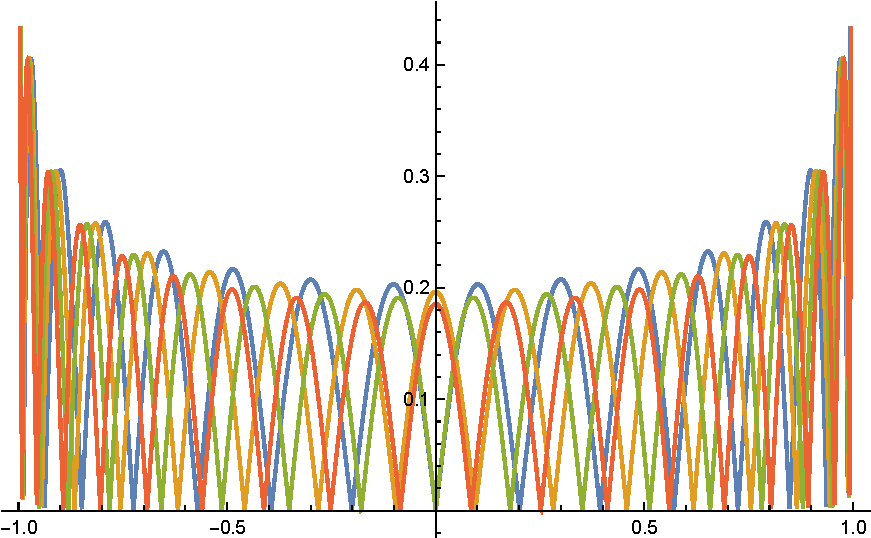
\includegraphics{amplitude_response.pdf}}
\caption{Amplitude response}
\label{fig:amp_response}
\end{figure}

In signal processing, a comb filter adds a delayed version of a signal to itself, causing constructive and destructive interference.
This can be viewed as a feedforward comb filter.

\bibliography{../../bibliography}

\end{document}